\chapter{Аналитическая часть}
В данном разделе рассмотрена информация, касающаяся основ конвейерной обработки данных.

\section{Конвейерная обработка данных}
Конвейер~\cite{conway} \text{(англ. \textit{conway})} --- организация вычислений, при которой увеличивается количество выполняемых инструкций за единицу времени за счет использования принципов параллельности.

Конвейеризация (или конвейерная обработка) в общем случае основана на разделении подлежащей исполнению функции на более мелкие части, называемые ступенями, и выделении для каждой из них отдельного блока аппаратуры. 
Так, обработку любой машинной команды можно разделить на несколько этапов (несколько ступеней), организовав передачу данных от одного этапа к следующему. 
При этом конвейерную обработку можно использовать для совмещения этапов выполнения разных команд. 
Производительность при этом возрастает, благодаря тому, что одновременно на различных ступенях конвейера выполняется несколько команд. 
Конвейерная обработка такого рода широко применяется во всех современных быстродействующих процессорах.

Конвейеризация позволяет увеличить пропускную способность процессора (количество команд, завершающихся в единицу времени), но она не сокращает время выполнения отдельной команды. 
В действительности она даже несколько увеличивает время выполнения каждой команды из-за накладных расходов, связанных с хранением промежуточных результатов. 
Однако увеличение пропускной способности означает, что программа будет выполняться быстрее по сравнению с простой, не конвейерной схемой.


\section{Разреженный строчный формат матрицы}

Во многих областях человеческой деятельности информацию
часто представляют в форме матриц. Матрица --- это регулярный
числовой массив. Разреженная  матрица --- матрица, в которой большинство элементов равны нулю.

Разреженный строчный формат (сокр. РСФ)~\cite{csr} --- это одна из наиболее широко используемых схем хранения разреженных матриц.
Эта схема предъявляет минимальные требования к памяти и в то же
время оказывается очень удобной для нескольких важных операций над разреженными матрицами: сложения, умножения,
перестановок строк и столбцов, транспонирования, решения линейных систем с разреженными матрицами коэффициентов как
прямыми, так и итерационными методами и т. д. 
Значения ненулевых элементов матрицы и соответствующие столбцовые индексы хранятся в этой схеме по строкам в двух массивах; назовем их соответственно $AN$ и $JA$. 
Используется также массив указателей (скажем, $AI$, еще обозначающийся как $NR$), отмечающих позиции массивов $AN$ и $JA$, с которых начинается описание очередной строки. Дополнительная компонента в $AI$ содержит указатель первой свободной позиции в $JA$ и $AN$. 
Пример представления матрицы РСФ на рисунке~\ref{fig:ex-csr}.

\begin{figure}[h]
	\centering
	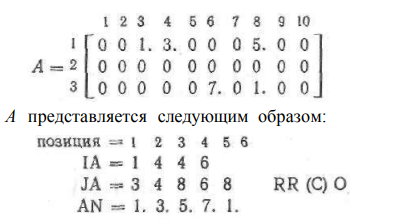
\includegraphics[width=0.85\textwidth]{img/example_csr.png}
	\caption{Пример представления матрицы в РСФ}
	\label{fig:ex-csr}
\end{figure}

В общем случае описание i-й строки $А$ хранится в позициях с $IA(i)$ до $IA(i + 1)$ --- 1 массивов $JA$ и $AN$, за исключением
равенства $IA(i + 1) = IA(i)$, означающего, что r-я строка пуста.
Если матрица $А$ имеет $n$ строк, то $IA$ содержит $n + 1$ позиций. 

\section{Сложение РСФ матриц}

Для сложения матриц в РСФ необходимо пройти через матрицу указателей $AI$ поэлементно через две матрицы, выделяя интервалы между соседними элементами $AI$ по $AN$ и $JA$, то есть $AI(i)$ и $AI(i + 1)$.
Если встретится элементы с одинаковыми строками и столбцами, то производится сложение. Затем происходит повторные проходы по двум матрицам  по отдельности для того чтобы добавить в результирующую матрицу остаточные значение~\cite{csr}.

\section{Описание алгоритмов}

В качестве операций, выполняющихся на конвейере, взяты следующие:
\begin{enumerate}
	\item создание двух матриц в РСФ;
	\item сложение двух созданных ранее матриц в РСФ;
	\item распаковка результата РСФ в классическое матричное представление.
\end{enumerate}

Ленты конвейера (обработчики) будут передавать друг другу заявки. Первый этап, или обработчик, будет формировать заявку, которая будет передаваться от этапа к этапу

Заявка будет содержать:
\begin{itemize}
	\item две матрицы в РСФ;
	\item результат сложения двух матриц в РСФ;
	\item матрица в классическом представлении для распаковки;
	\item временные отметки начала и конца выполнения стадии обработки заявки.
\end{itemize}

\section*{Вывод}
В данном разделе было рассмотрено понятие конвейерной обработки, а также выбраны этапы для обработки матрицы, которые будут обрабатывать ленты конвейера. Также рассмотрена разреженная матрицы и операция сложения таких матриц.

Программа будет получать на вход количество задач, размеры матрицы и количество ненулевых элементов, а также выбор алгоритма --- линейный или конвейерный.

Реализуемое программное обеспечение будет давать возможность получить журнал программы для установленного числа задач при линейной и конвейерной обработке. 
Также будет возможность провести тестирование по времени для разного количества задач и разных размеров самих матриц.